%%%%%to do list %%%%%%

% 1. change arrow size in uni and bi directional pictures by using arrows.meta


%%%%%%%%%%%%%%%%%%%%%%%%%%%%%%%%%%%%%%
% LaTeX poster template
% Created by Nathaniel Johnston
% August 2009
% http://www.nathanieljohnston.com/2009/08/latex-poster-template/
%%%%%%%%%%%%%%%%%%%%%%%%%%%%%%%%%%%%%%

\documentclass[final]{beamer}
\usepackage{etex}

\usepackage[scale=1.25]{beamerposter} 
\newcommand{\diag}{\mbox{{\rm diag}}}
\usepackage[labelformat=simple]{subcaption}
\renewcommand\thesubfigure{(\alph{subfigure})}
\captionsetup{compatibility=false}
\usepackage{pgfplots, graphicx,verbatim, amsmath,amsthm,amssymb,mathtools,   natbib,tikz} 

\usetikzlibrary{arrows,snakes,backgrounds,shapes, decorations.markings}
\usetikzlibrary{matrix}
\usetikzlibrary{chains}
\usetikzlibrary{positioning}
\usetikzlibrary{arrows.meta}


%-----------------------------------------------------------
% Define the column width and poster size
% To set effective sepwid, onecolwid and twocolwid values, first choose how many columns you want and how much separation you want between columns
% The separation I chose is 0.024 and I want 4 columns
% Then set onecolwid to be (1-(4+1)*0.024)/4 = 0.22
% Set twocolwid to be 2*onecolwid + sepwid = 0.464
%-----------------------------------------------------------

\newlength{\sepwid}
\newlength{\onecolwid}
\newlength{\twocolwid}
\newlength{\threecolwid}
\setlength{\paperwidth}{48in}
\setlength{\paperheight}{36in}
%four columns settings
%\setlength{\sepwid}{0.024\paperwidth}
%\setlength{\onecolwid}{0.22\paperwidth}
%\setlength{\twocolwid}{0.464\paperwidth}
%\setlength{\threecolwid}{0.708\paperwidth}
%\setlength{\topmargin}{-0.5in}

%three columns settings
\setlength{\sepwid}{0.024\paperwidth}
\setlength{\onecolwid}{0.3013\paperwidth}
\setlength{\twocolwid}{0.626\paperwidth}
\setlength{\threecolwid}{0.626\paperwidth}
\setlength{\topmargin}{-0.5in}

%major theme colors
\usetheme{confposter}
\usepackage{exscale}

%-----------------------------------------------------------
% The next part fixes a problem with figure numbering. Thanks Nishan!
% When including a figure in your poster, be sure that the commands are typed in the following order:
% \begin{figure}
% \includegraphics[...]{...}
% \caption{...}
% \end{figure}
% That is, put the \caption after the \includegraphics
%-----------------------------------------------------------

\usecaptiontemplate{
\small
\structure{\insertcaptionname~\insertcaptionnumber:}
\insertcaption}

%-----------------------------------------------------------
% Define colours (see beamerthemeconfposter.sty to change these colour definitions)
%-----------------------------------------------------------

\setbeamercolor{block title}{fg=SFUred,bg=white}
\setbeamercolor{block body}{fg=black,bg=white}
\setbeamercolor{block alerted title}{fg=white,bg=SFUred}
\setbeamercolor{block alerted body}{fg=black,bg=SFUred!10}

%make sure figures are numbered
\setbeamertemplate{caption}[numbered]

%define theorem environments
\setbeamertemplate{theorems}[numbered]
\newtheorem{proposition}[theorem]{Proposition}

%-----------------------------------------------------------
% Name and authors of poster/paper/research
%-----------------------------------------------------------

\title{A Neural Network Approach to Classifying Banana Ripeness}
\author{Kyle Demeule (kdd2@sfu.ca), Bernard S Chan (bernardc@sfu.ca), Saeed Soltani (saeeds@sfu.ca)}
\institute{Department Computing Science, Faculty of Applied Sciences, Simon Fraser University}

%-----------------------------------------------------------
% Start the poster itself
%-----------------------------------------------------------
\usepackage{gensymb}
\begin{document}
\begin{frame}[t]
  \begin{columns}[t]												% the [t] option aligns the column's content at the top
    \begin{column}{\sepwid}\end{column}			% empty spacer column
    \begin{column}{\onecolwid}
%      \begin{block}{Purpose}
%        Our purpose in this work is to investigate Hamiltonian coupled cell systems. Particularly, we are interested in the effects of coupling functions and coupling topology on the dynamics of the network. 
   %   \end{block}
      %\vskip2ex
\begin{block}{Introduction}
\begin{itemize}
\item Interested in classifying fruit ripeness using machine learning methods. 
\item Previously studied by~\citet{saad2009recognizing} through neural network methods. 
\item More than just bananas: Aim to improve upon previous work by incorporating non-banana objects. 
\item Previous data set unavailable; will establish our own data set. 

\end{itemize}
\end{block} %introduction block
            \vskip2ex
\begin{alertblock}{Data Collection}
\begin{itemize}
\item Generated the data set by taking pictures of bananas and objects that are not bananas.
\item Lighting, camera (Canon S90) and background were controlled. 
\item Used 12 unique bananas at various stages to represent the three stages ripeness: 
\begin{enumerate}
\item pre-ripe, 
\item ripe, and 
\item rotten. 
\end{enumerate}
\item Used green pepper, apple, tomato, lemon and lime as non-banana objects. 
\item Pictures were resized and cropped to a square. 
\item Incorporated each picture at $0\,^{\circ}$, $90\,^{\circ}$, $180\,^{\circ}$ and  $270\,^{\circ}$ of rotation to increase the number of pictures in the data set by four fold.
\end{itemize}
\end{alertblock}
 \vskip1ex
 \begin{figure}
  \begin{subfigure}{.28\textwidth}
  \centering
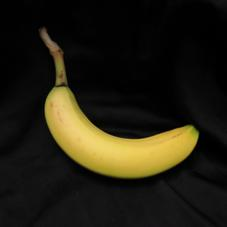
\includegraphics[width=\textwidth]{1_preripe.jpg}
\caption{}
\label{fig;preripe}
\end{subfigure}%
\quad
 \begin{subfigure}{.28\textwidth}
  \centering
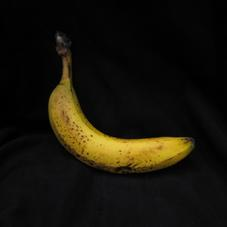
\includegraphics[width=\textwidth]{2_ripe.jpg}
\caption{}
\label{fig:ripe}
\end{subfigure}%
\quad
  \begin{subfigure}{.28\textwidth}
  \centering
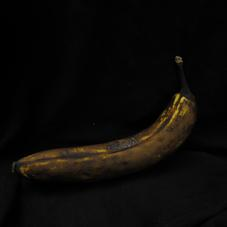
\includegraphics[width=\textwidth]{0_overripe.jpg}
\caption{}
\label{fig:overripe}
\end{subfigure}%
\caption{  (a) Pre-ripe banana. (b) Ripe banana. (c) Overripe banana.}
\end{figure}
\end{column}

    \begin{column}{\sepwid}\end{column}			% empty spacer column


        \begin{column}{\onecolwid}

          
 \begin{block}{Tools and Methods}
 \begin{itemize}
 \item Caffe.
 \item AlexNet.
 \item SciKit Learn: a Python library of machine learning algorithms. 
 \end{itemize}
 
 
  \end{block} %tools and methods block
         
%         \begin{theorem}\label{linearHamiltonianTheorem}
\vskip1ex

\begin{alertblock}{Features Extraction via AlexNet}
\end{alertblock}
\vskip1ex

\begin{block}{Experimental Results}
      
\end{block}
 \end{column}
  \begin{column}{\sepwid}\end{column}			% empty spacer column        
  
        \begin{column}{\onecolwid}
        

%        \begin{theorem}
\begin{block}{Results}

\vskip1ex

\begin{alertblock}{General Nonlinear Criteria}
\end{alertblock}
Based on all aforementioned criteria, the digraph in Figure~\ref{fig:example1} is a nontrivial  example that would admit a general nonlinear Hamiltonian coupled cell system.  
\end{block}
\begin{block}{Conclusion and Potential Applications}
\begin{itemize}
\item Able to enhance previous work by adding non-banana objects. 
\item Working towards generalizing ripeness detection for fruits, vegetable and other in general. 
\item Industrial application: automatic large scale sorting of fruits and vegetable based on ripeness and type. 
\item Mobile app for visually disabled: quickly find the ripeness of fruits and vegetables via machine learning model. 
\end{itemize}
\end{block}
%\vskip1ex
\begin{block}{Acknowledgement}
We want to thank our TA Zhiwei (Lucas) Deng for his suggestions and guidance on using Caffe as well as AlexNet. Furthermore, we want to thank Dr. Mori for his insights and suggestions on this project. 
\end{block}
          \begin{block}{References}
   \bibliography{poster}		    
   \bibliographystyle{abbrvnat}
  \end{block}
  \vskip1ex
  \begin{figure}
  \centering
  
\includegraphics[width=.9\textwidth]{SFU_StdTag-Horz_Pos_CMYK.eps}
  \end{figure}
    \end{column}

 \end{columns}
\end{frame}
\end{document}
